
\newcommand{\CanTableNote}{$LEAP$ is the Longitudinal Employment Analysis Program and $CanSynLBD$ is the Canadian synthetic database based on LEAP. }

\subsection{Entity Characteristics}

The CanSynLBD and LEAP generally provide comparable inferences on aggregate means and correlations. For example, 
%Figures \ref{tab:Can:GrossEmploymentPrivate} and \ref{tab:Can:GrossEmploymentManufacturing} 
Panels a and b of Figure~\ref{tab:all:characteristics}
show that gross employment levels for each year in the CanSynLBD are very close to those in the LEAP. However, the manufacturing sector shows closer patterns than the private sector.\footnote{The private sector comprises all industries including the manufacturing sector except the public sector  (NAICS 61, 62, and 91)} We find similar results for total payroll (Panels c and d of Figure~\ref{tab:all:characteristics}).
  %Figures \ref{tab:Can:TotalPayrollPrivate} and  \ref{tab:Can:TotalPayrollManufacturing}) .

\begin{figure} [H]
\centering
\label{tab:all:characteristics}
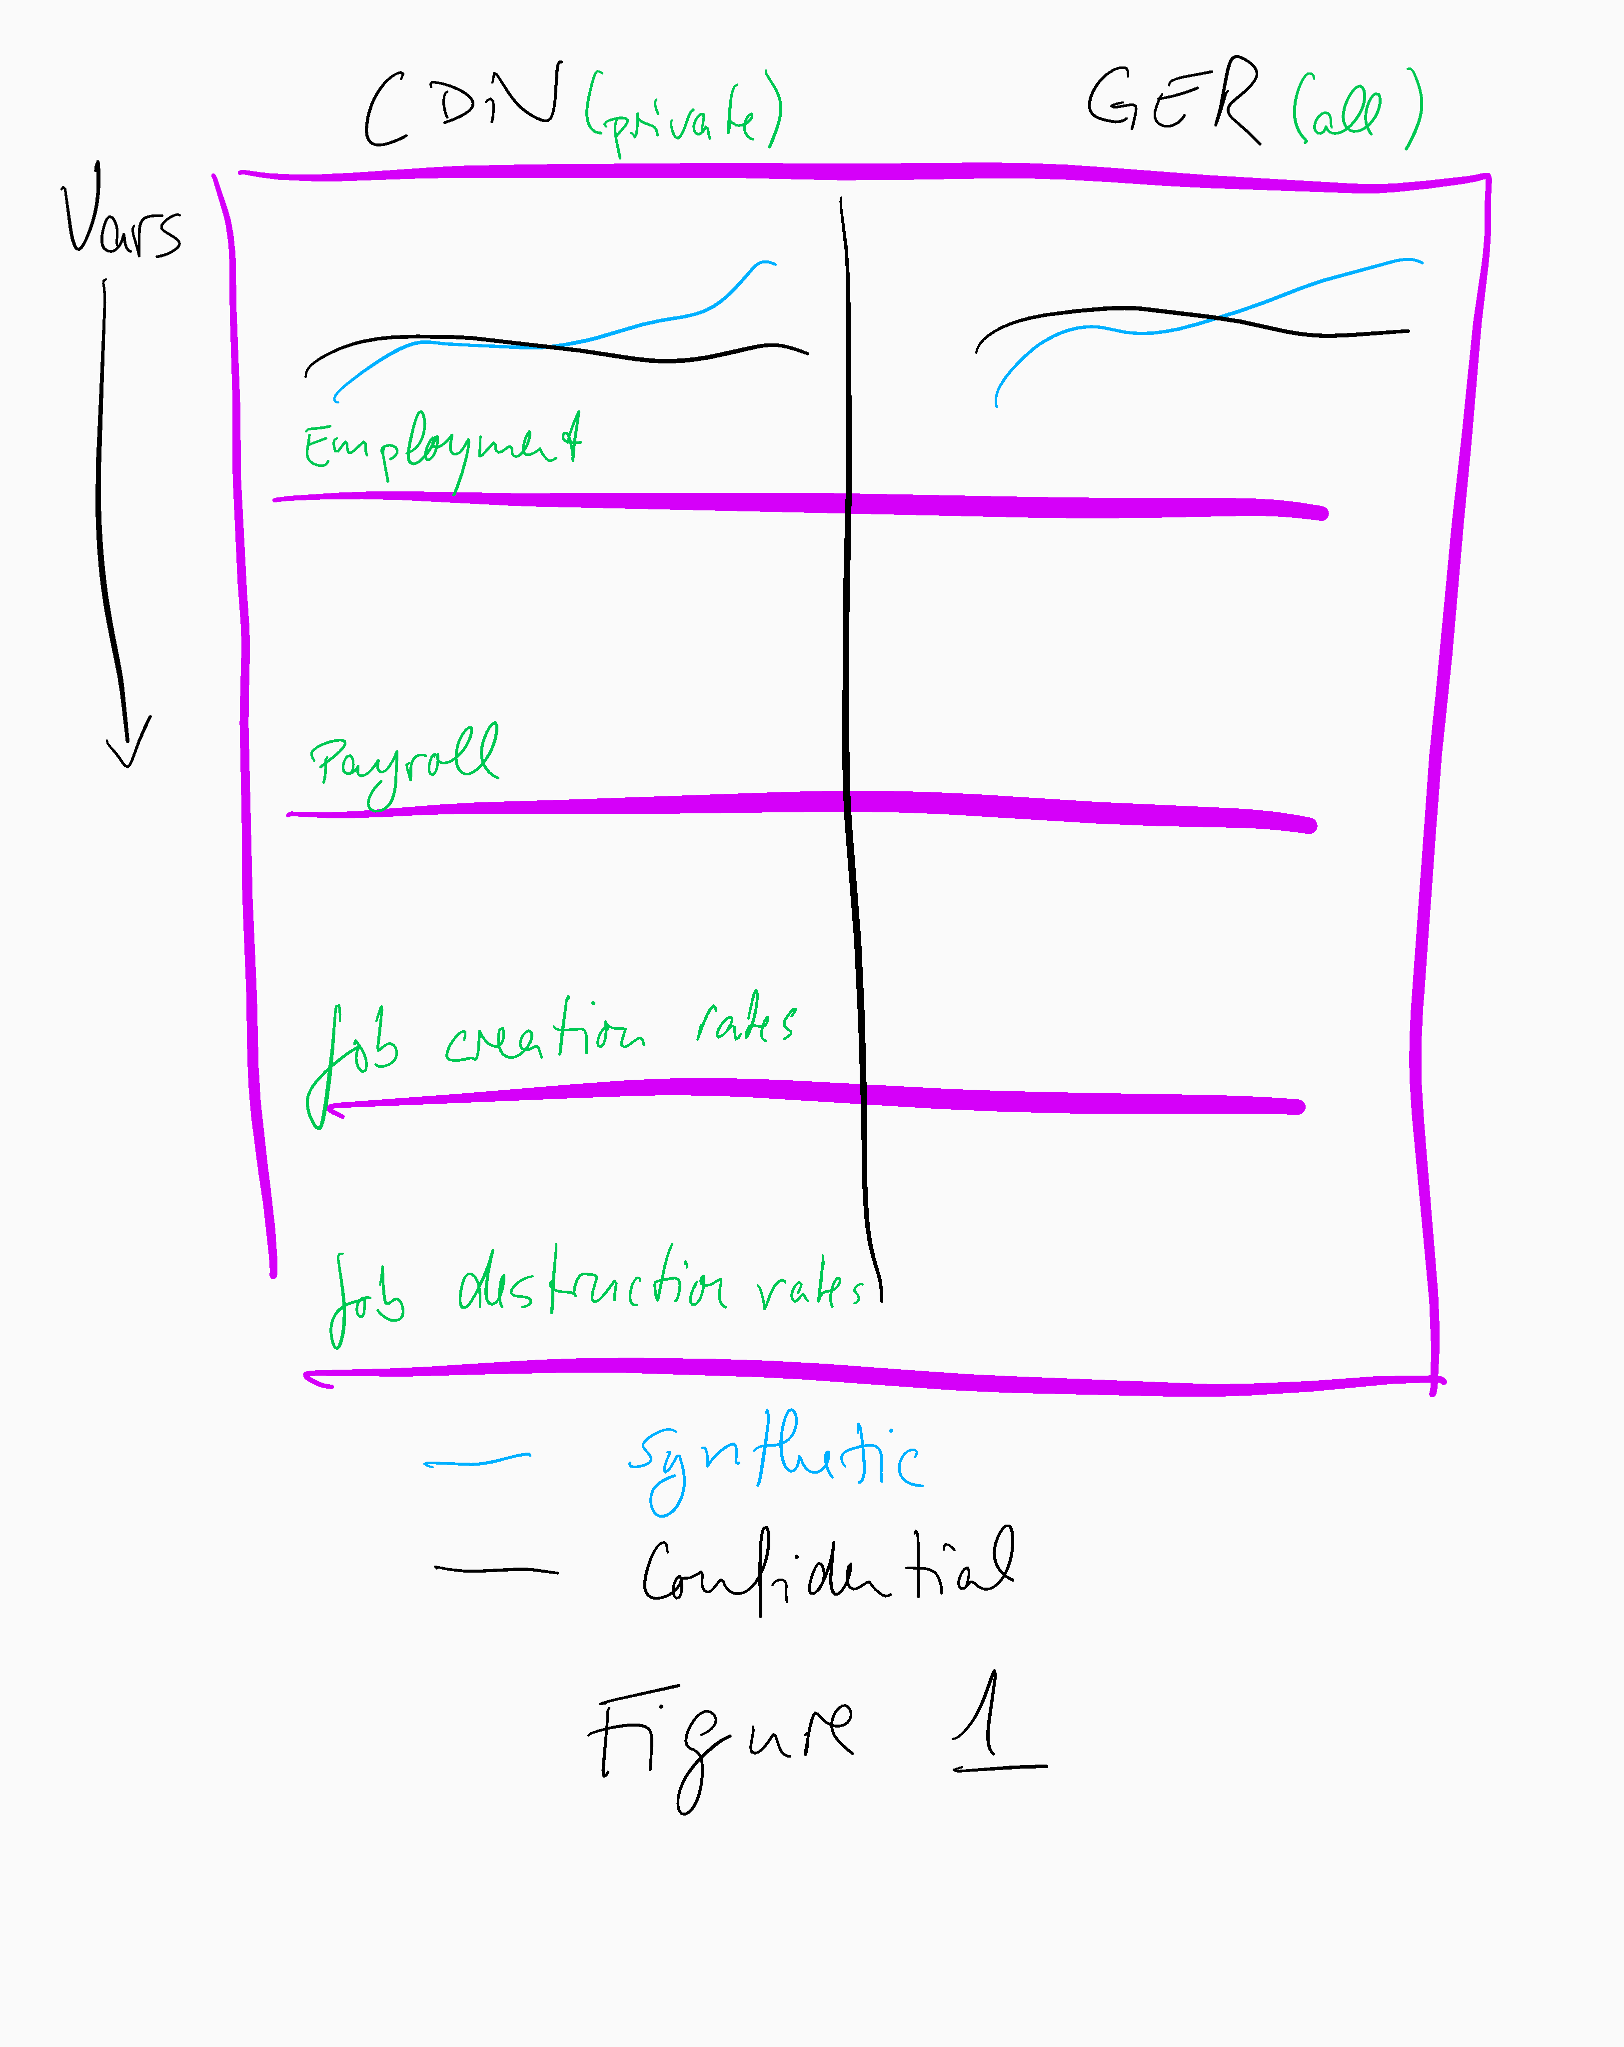
\includegraphics[width=.8\linewidth]{graphs/Figure1-placeholder.png} 
\caption{Alternate graph} 
\begin{minipage}{0.48\linewidth}
{\footnotesize To be computed in R, or redone in Stata using GPH files. \par}
\end{minipage}
\end{figure}


\subsection{Dynamics of Job Flows}

One of the most important applications of LEAP is to generate statistics that describe job flows. Following \cite{DavisHaltiwangerSchuh}, the job creation is defined as the sum of all employment gains from expanding firms from year $t-1$ to year $t$ including entry firms. The job destruction rate is defined as the sum of all employment losses from contracting firms from year $t-1$ to year $t$ including exiting firms. Net job creation is the job creation rate minus the job destruction rate. Figures \ref{JobCreationPrivate} and \ref{JobCreationManufacturing} show the job creation rates from the CanSynLBD compared againg those of the LEAP. These figures show that the manufacturing sector has closer pattern than the private sector. We find a similar patterns for net job creation rates (Panels x and y of Figures \ref{NetJobCreationPrivate} and  \ref{NetJobCreationManufacturing}).



\subsection{Entity Dynamics}
To assess how well the synthetic data capture entity dynamics, we also compute entry and exit rates  by year. Table \ref{tab:Can:FirmDynamics} shows that those rates for CanSynLBD are similar to LEAP database. To show further those rates are similar, we compute the divergence of entry rate as the entry rate of CanSynLBD net the entry rate of LEAP as well as the divergence of exit rate as the exit rate of CanSynLBD net the exit rate of LEAP (see Figure \ref{Divergence}).

\todo{Also consolidate graphs here}
\begin{figure} [H]
\centering
\label{tab:Can:FirmDynamics}
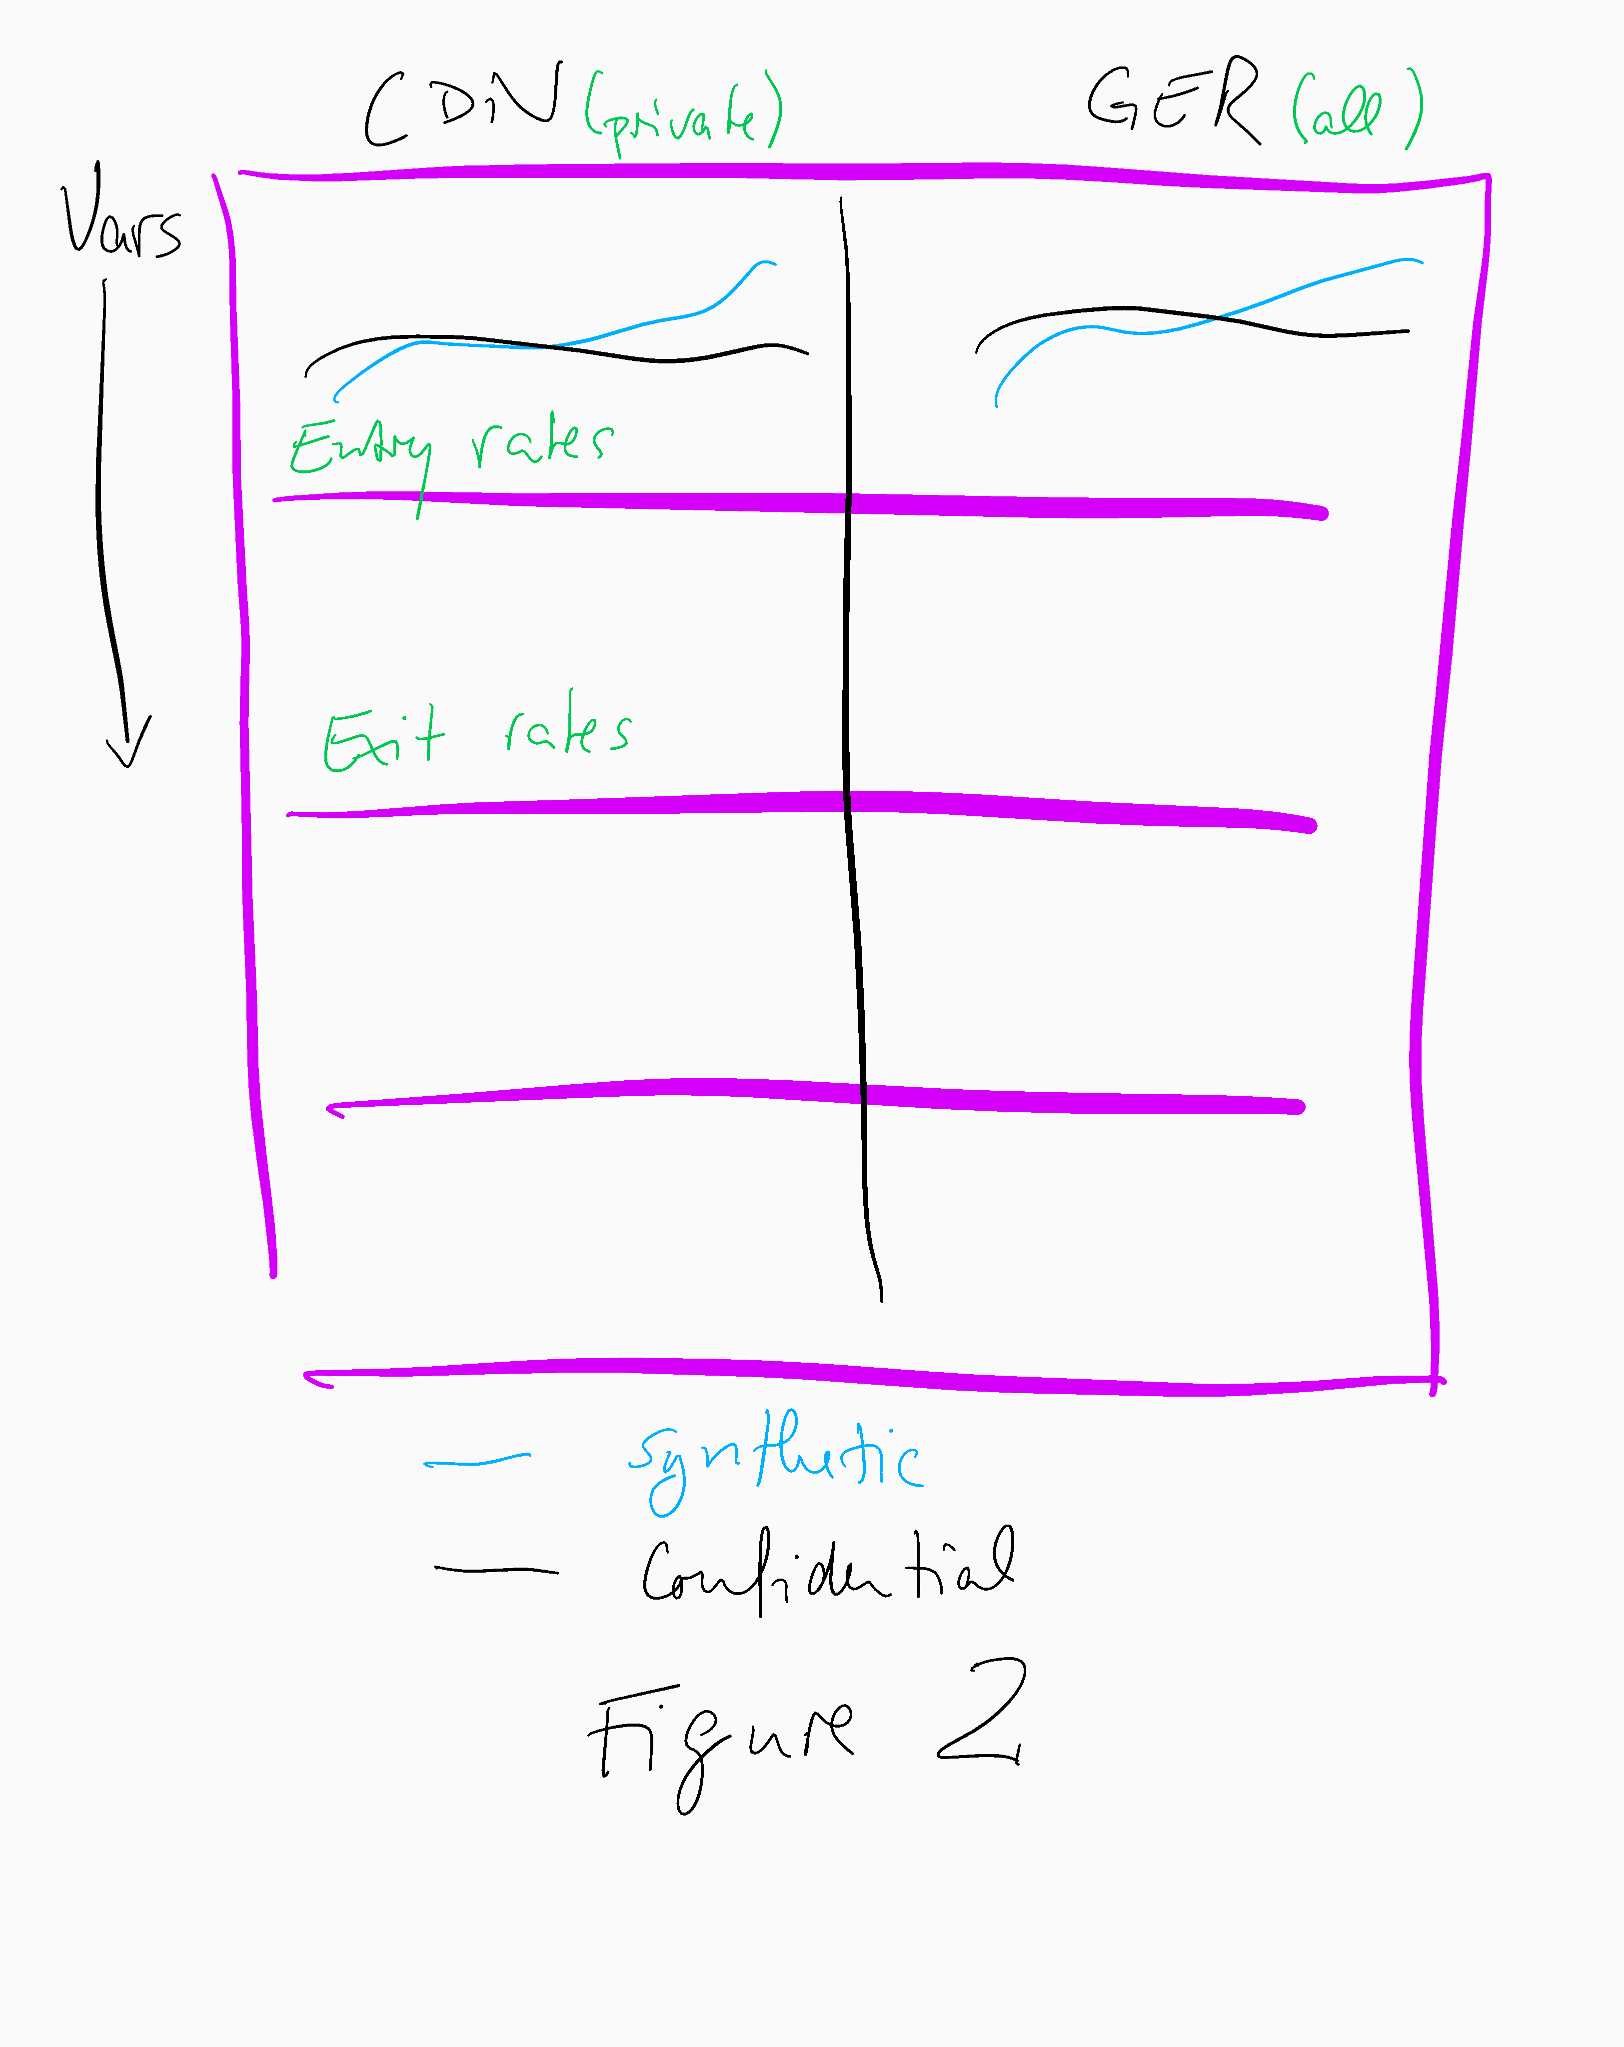
\includegraphics[width=.8\linewidth]{graphs/Figure2-placeholder.png} 
\caption{Alternate graph} 
\begin{minipage}{0.48\linewidth}
{\footnotesize To be computed in R, or redone in Stata using GPH files. Detailed data are in the appendix. \par}
\end{minipage}
\end{figure}


\subsection{Distribution of variables across time and industry}

\SynLBD{} keeps fixed the total number of entities that ever exist within the time frame used, but because each entity's entry and exit date are synthesized, the total number of entities at a particular point in time may differ, and with it employment and payroll. We inspect this distribution in the Canadian data, by industry, in the following figures.\footnote{Since the German data was only generated for a very small number of industries, we skip this step for Germany.} 


Figures~\ref{FirmSharePrivate} and \ref{FirmShareManufacturing} plot the share of firms by two-digit industry and year for both the Canadian synthetic  and confidential data. If only contemporaneous features (employment, payroll), and birth and death of the synthetic entities were the same, all observations would be on the 45 degree line. The figures show some divergence of the within-industry distribution across time. 


Given a distribution of entities alive, we can also compute the share of observed characteristics across time and industry. Shares of a variable $X$ are computed as a fraction of the sum of $X$ across \textit{all} years and industries:

\begin{equation}
    \label{eq:share_employment}
x_{its} = X_{its}/\sum_{i} \sum_{t} X_{its}, 
\end{equation}

where $i$ are two-digit industries, $t$ are  years in-sample, $s$ indicates whether it is in the synthetic or confidential data, and $X_{its}$ is the sum of the variable of interest $X$ for industry $i$ and year $t$ in  dataset $s$.

\todo{Also consolidate graphs here}
\begin{figure} [H]
\centering
\label{tab:all:shares}
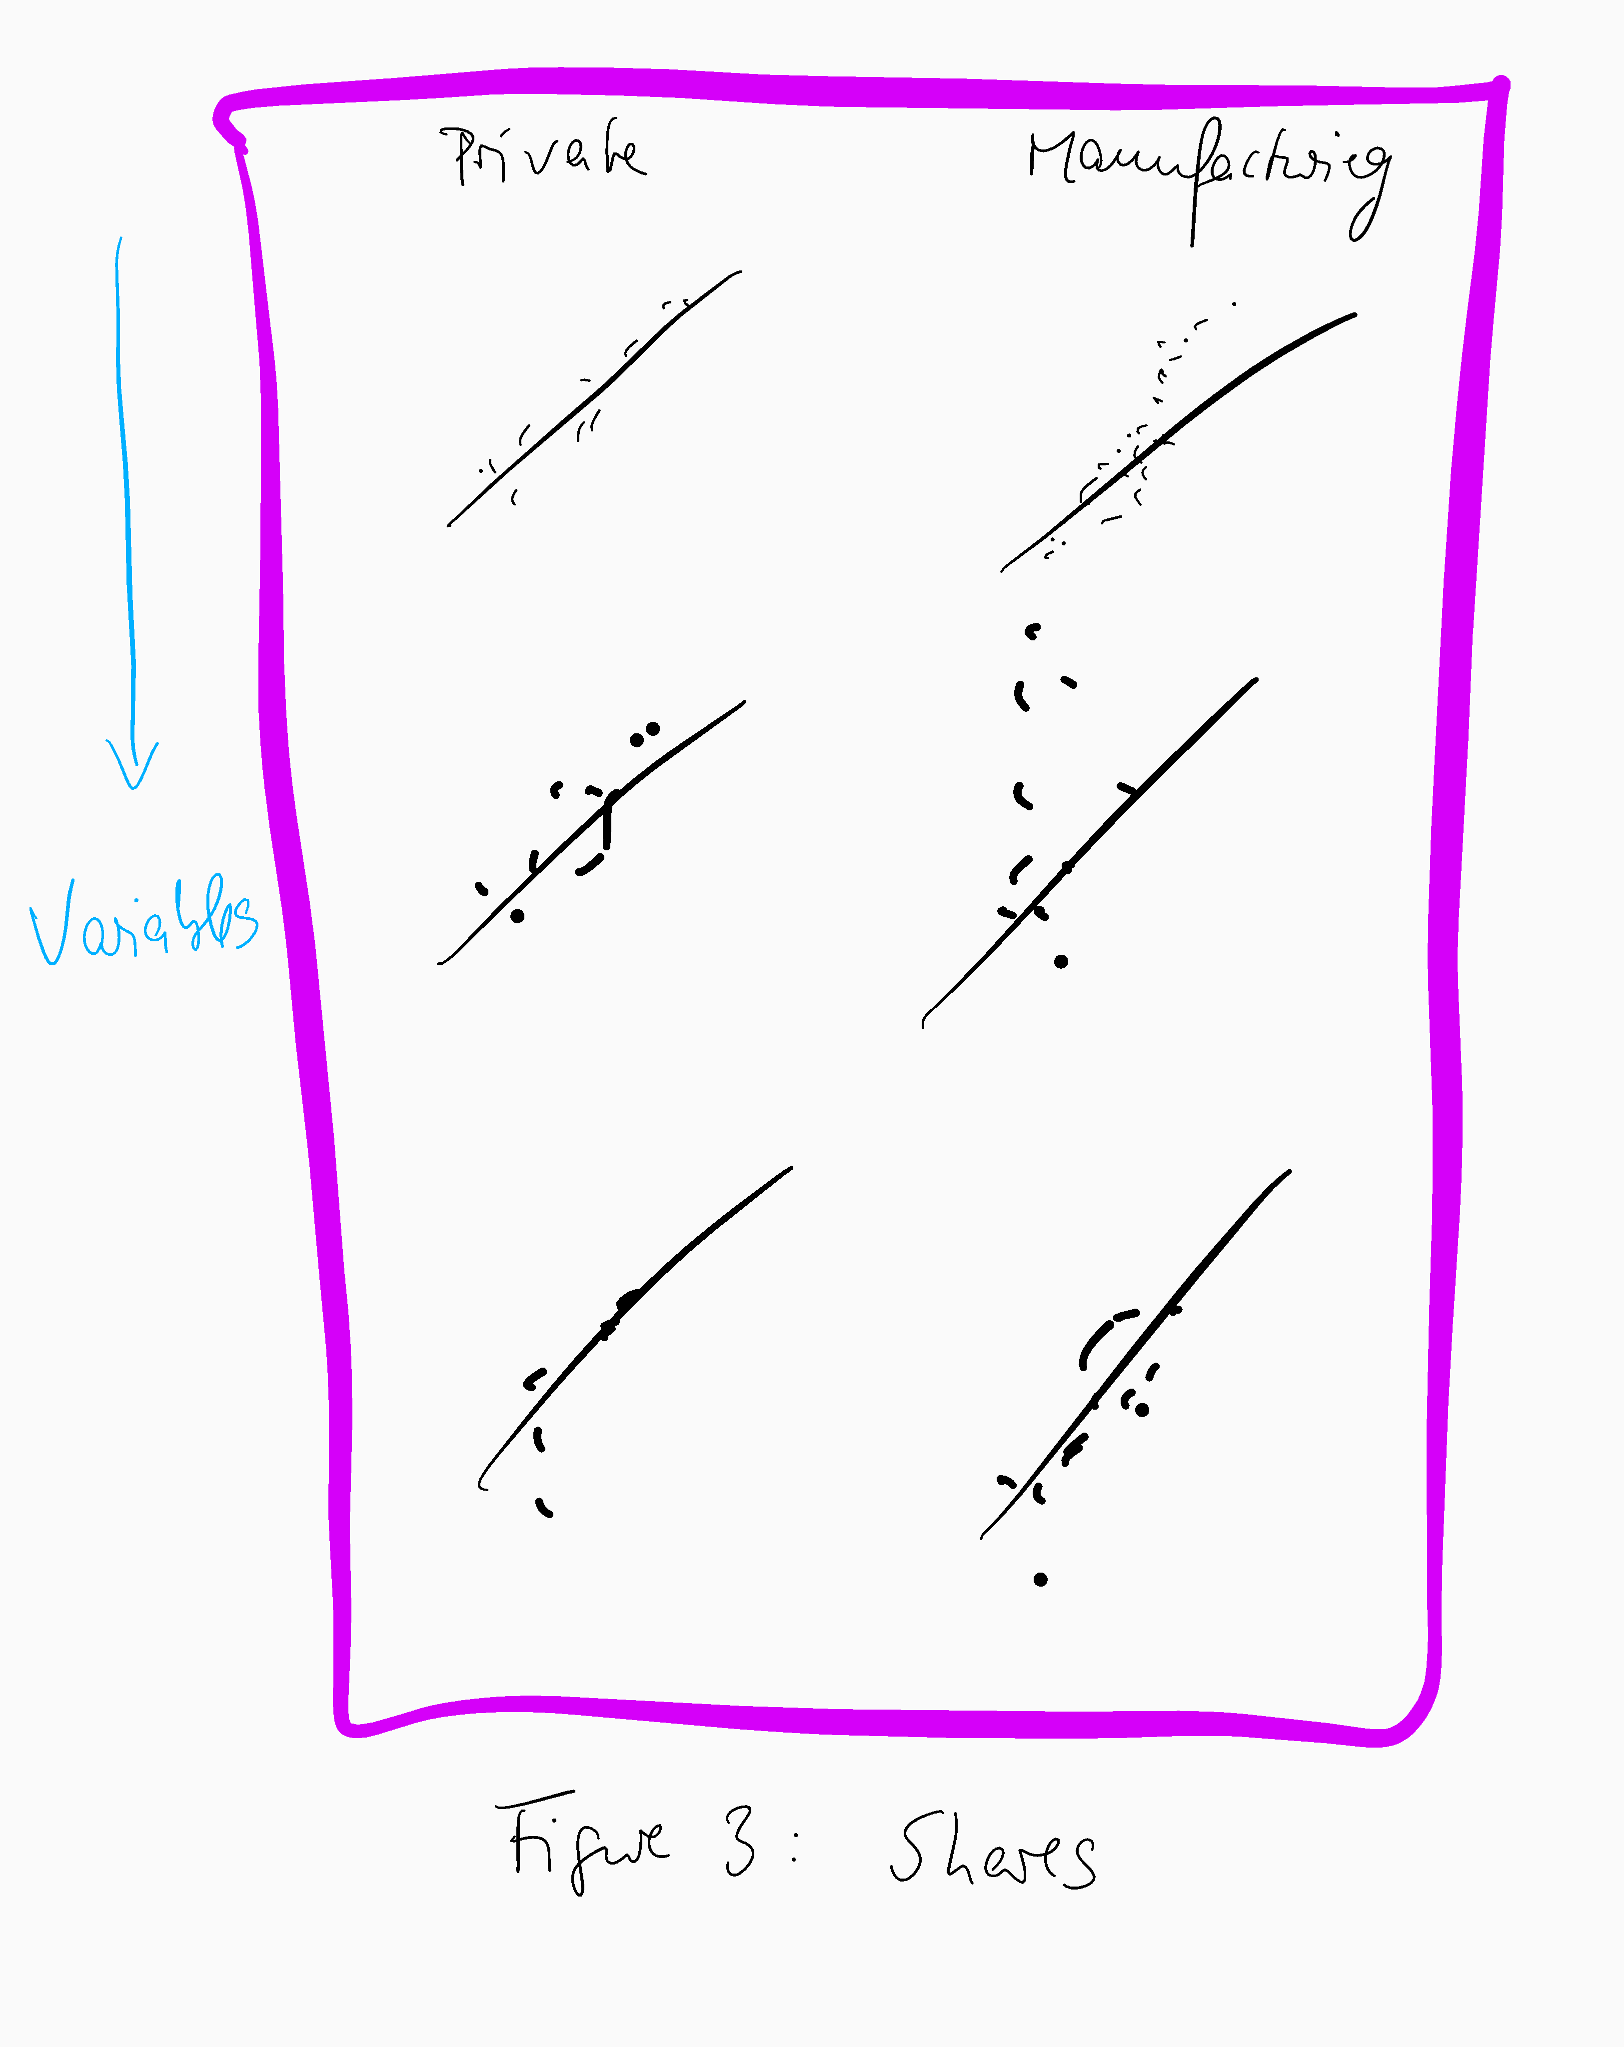
\includegraphics[width=.8\linewidth]{graphs/Figure3-placeholder.png} 
\caption{Alternate graph} 
\begin{minipage}{0.48\linewidth}
{\footnotesize To be computed in R, or redone in Stata using GPH files. Detailed data are in the appendix. \par}
\end{minipage}
\end{figure}


Figures~\ref{EmploymentSharePrivate} and \ref{EmploymentShareManufacturing} plot the share of employment by two-digit industry and year for both  CanSynLBD and the LEAP database. 
Employment shares  do not cluster along the 45-degree line. However, this hides significant differences between sectors. For instance,  the share of employment for the manufacturing sector does show stronger clustering along the 45-degree line.

\
Figures~\ref{PayrollSharePrivate} and~\ref{PayrollShareManufacturing} plot the share of \textit{payroll} by two-digit industry and year for both CanSynLBD and LEAP database. In general, shares do not cluster along the 45-degree line, though a focus on  the manufacturing sector again shows stronger clustering along the 45-degree line.


\subsection{pMSE}


To compute the $pMSE$, we estimate equation \ref{pMSE} using both the logit and probit models. TTable~\ref{tab:pMSE_regression} shows the results from the estimation of $pMSE$ for the Canadian data.
\todo{BD: Are those coefficients or marginal effects? Does it make sense to show coefficients? Or are we interested only in the last row? If we are interested in the coefficient, why is there no discussion of those?} 
\todo{Those are coefficients. I think we are interested in the last row.} 
$pMSE$ is closer to zero for the manufacturing sector than the private sector in both regressions, consistent with our earlier observations for Canada.

%\newpage

DISCUSSION IS STILL MISSING.\todo{pMSE discussion}

\subsection{Regression Analysis}

\todo{Need to expand the regression discussion: only one generic model, many others possible, reference to the Singapore presentation by Lars}
To assess how well the synthetic data perform in a more complex model, we estimate four models similar to what users of the data (mostly economists) would use them for. This allows us to assess whether the synthetic data capture variability in economic growth due to industry and firm age.
The base model is  dynamic panel data model for the evolution of employment:

\begin{eqnarray}	
\label{eq:OLS}
Emp_{et} & = & \alpha + \theta Emp_{e,t-1} + \lambda Pay_{et} + Age_{et}^{T}\beta + \lambda_t + \alpha_i + \epsilon_{et}
\end{eqnarray}
where $Emp_{et}$ is log employment of entity $e$ in year $t$, $Emp_{e,t-1}$ is its one year lag, $Pay_{et}$ is the logarithm of payroll of entity $e$ in year $t$, $Age_{et}$ is a vector of dummy variables for age of entity $e$ in year $t$, $\lambda_t$ is the year fixed effect, $\alpha_i$ is an unobserved time-invariant industry-specific effect, and $\epsilon_{et}$ is the disturbance term of entity $e$ in year $t$. 

\todo{adjust for german analysis}
We estimate the model separately on confidential and synthetic data for the private sector (and for Canada, for the manufacturing sector). We find that the CansynLBD data provides similar predictions to LEAP data (Tables  \ref{OLS}).\todo{compute overlap interval} \todo{JA: @Lars, I think you mentioned once that you would like to calculate this. I could calculate using the method explained in the appendix.}



As $Emp_{e,t-1}$ is correlated with $\alpha_{i}$ because $Emp_{e,t-1}$ is a function of $\alpha_{i}$, \todo{This may need to be explained for non-economists - why is lagged employment of firm e a function of industry effect alpha i?}
OLS estimators are biased and inconsistent. 
To take this endogeneity bias into account, we use the estimation method from \textcite{RePEc:oup:restud:v:58:y:1991:i:2:p:277-297.} and find similar predictions (Table \ref{Dynamic - GMM}). To check the validity of the model, we use two tests. First, to test for autocorrelation, we use the test $m2$ by \textcite{RePEc:oup:restud:v:58:y:1991:i:2:p:277-297.}. In the table, we report the $z$ test statistic for $m2$ test for zero autocorrelation in the  first-differenced errors of order two. Second, we use the Sargan test to verify the validity of instrument subsets (shown in the last three rows in the table).

We furthermore estimate the model using the system GMM  method proposed by \textcite{RePEc:eee:econom:v:68:y:1995:i:1:p:29-51} and \textcite{RePEc:eee:econom:v:87:y:1998:i:1:p:115-143} and find similar predictions as before (detailed results in Table~\ref{Dynamic - system GMM}). 

We also estimate above dynamic panel data model with a first-order moving average using appropriate instruments for both level and difference equation as proposed by \textcite{RePEc:eee:econom:v:68:y:1995:i:1:p:29-51} and \textcite{RePEc:eee:econom:v:87:y:1998:i:1:p:115-143}:

\todo{@ JA: $\alpha$ is used twice - not clear - please verify - I have added subscripts}
\begin{eqnarray}	
Emp_{et}&=&\alpha_i +\theta Emp_{e,t-1}+\lambda Pay_{et}+Age_{et}^{T}\beta+\lambda_t+\alpha_i+\epsilon_{et}+\gamma\epsilon_{e,t-1}
\end{eqnarray}

Table~\ref{Dynamic - system GMM with MA(1)} shows that the CansynLBD provides similar predictions to the LEAP.

\todo{Also consolidate graphs here}
\begin{figure} [H]
\centering
\label{tab:all:estimates}
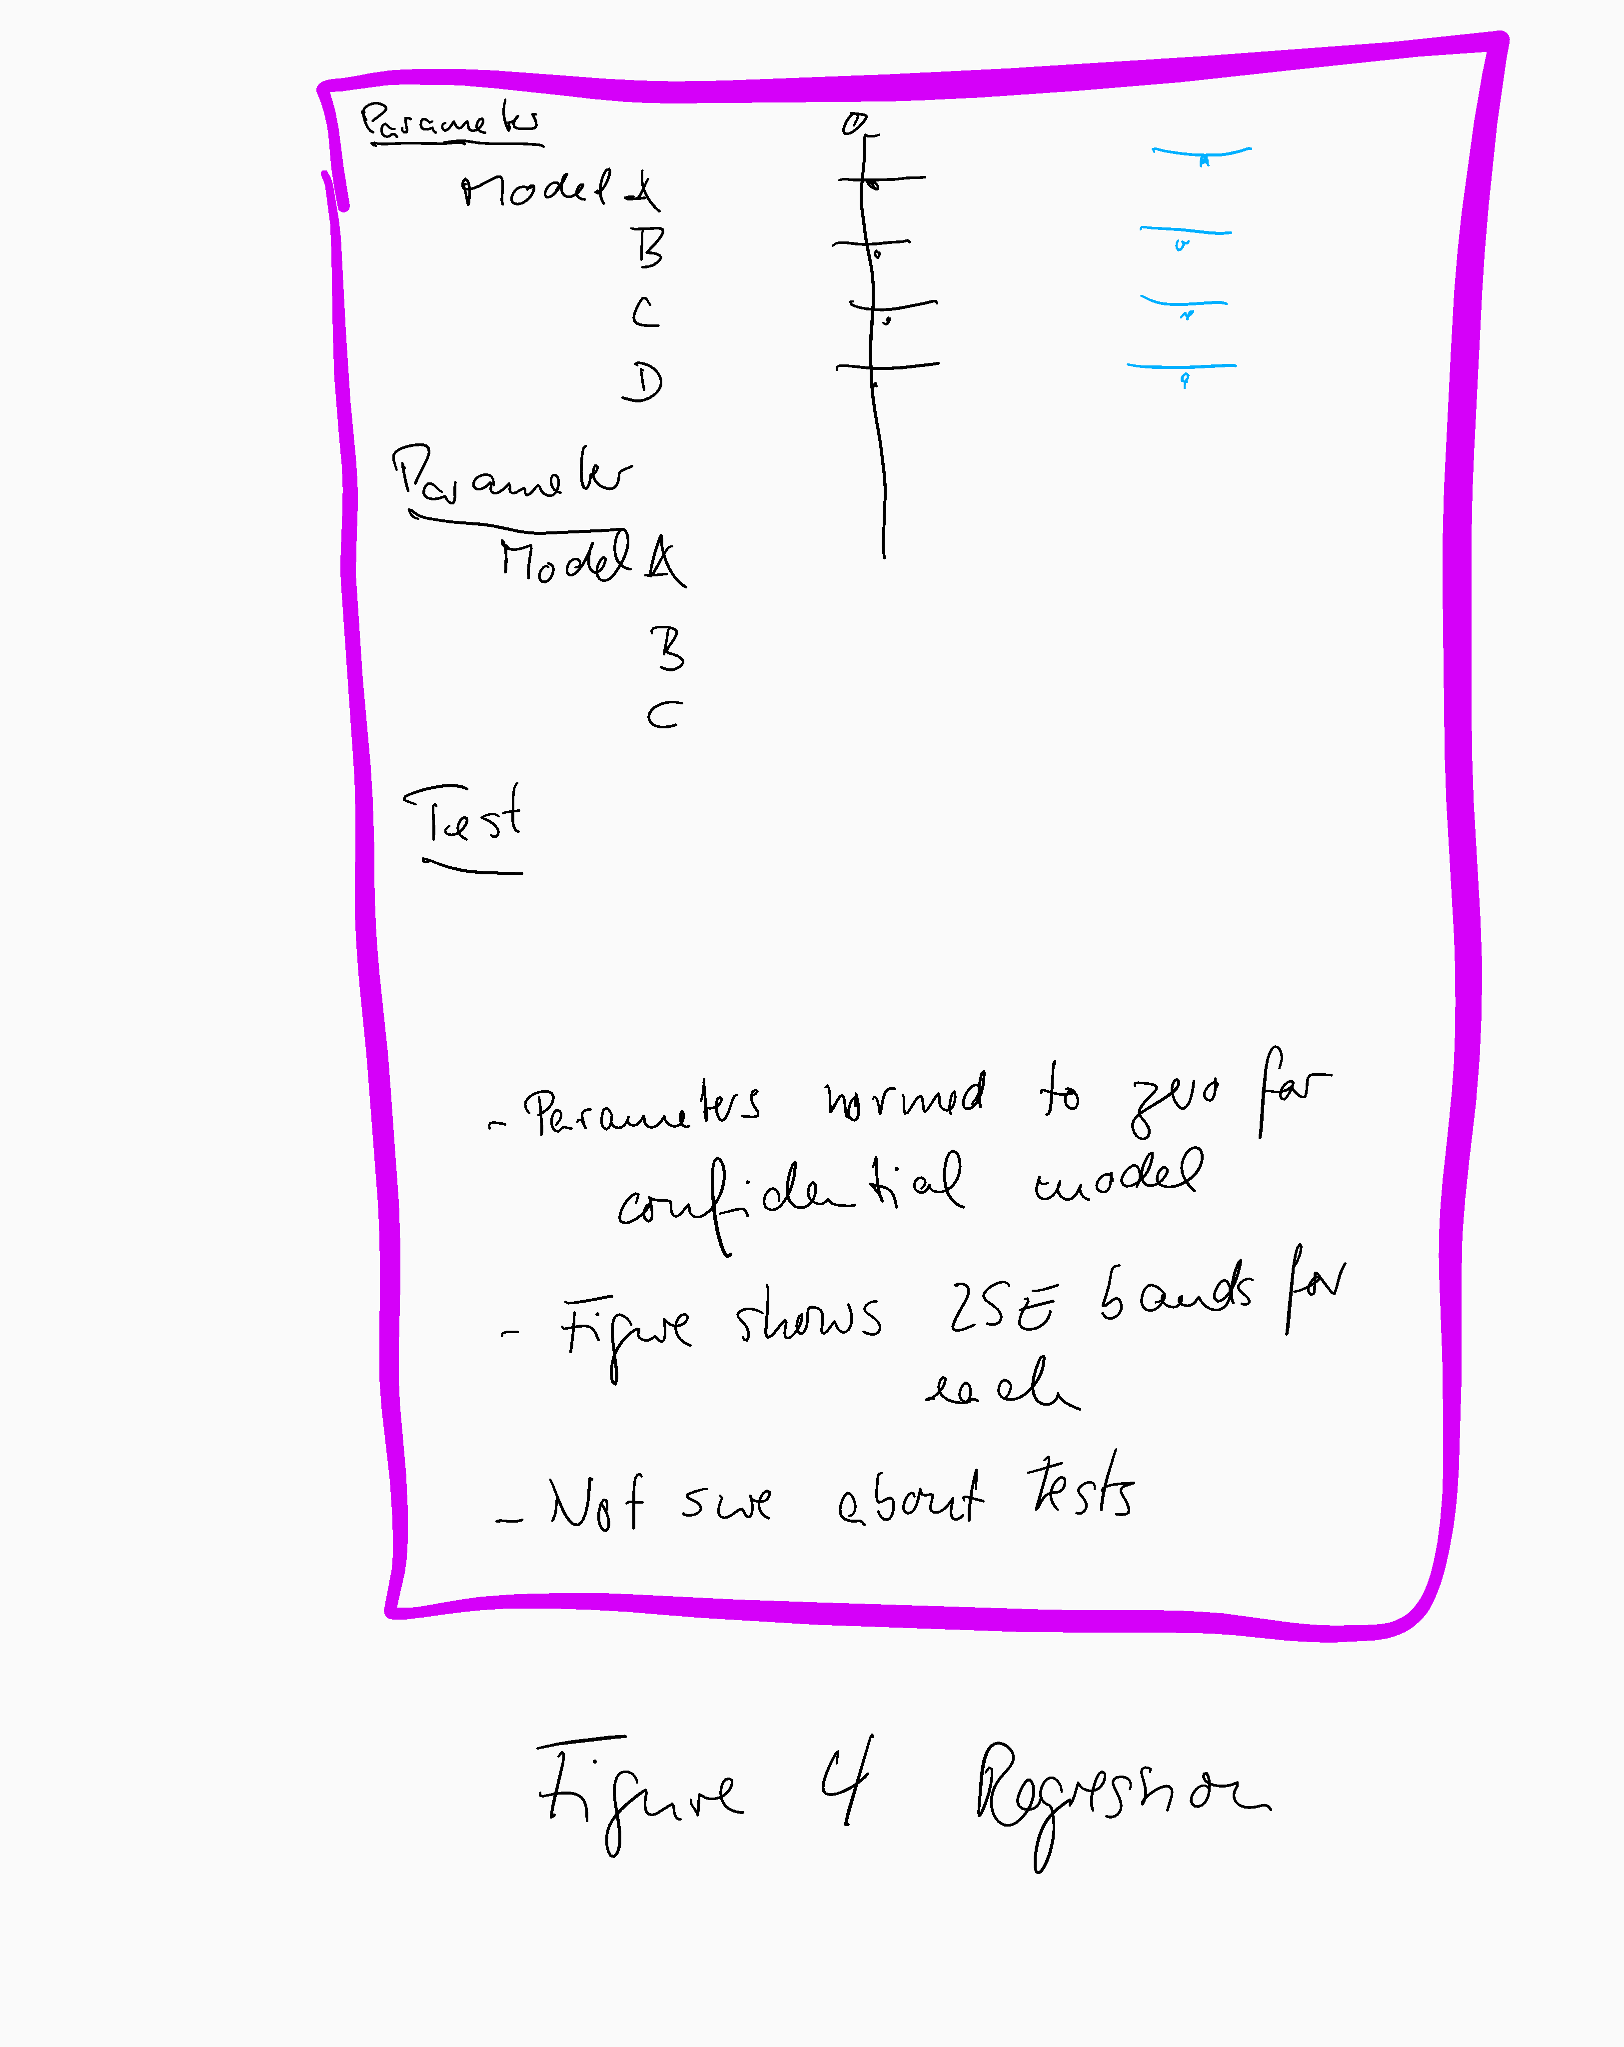
\includegraphics[width=.8\linewidth]{graphs/Figure4-placeholder.png} 
\caption{Alternate graph} 
\begin{minipage}{0.48\linewidth}
{\footnotesize To be computed in R. Detailed data are in the appendix. \par}
\end{minipage}
\end{figure}